% --------------------------------------------------------------------------------------------------
\section{Discussion and concluding remarks}
\begin{table}[H]
\centering \begin{tabular}{c|cc}
                                    & RMSE & Computation time\\\hline\hline
SARIMA (without covariates)         &  8.60 &  56 min \\
SARIMA (with covariates)            &  8.31 &  1h16   \\
Neural Network (without covariates) & 14.93 &  1h10   \\
Neural Network (with covariates)    & 10.29 &  40 min \\
XGBoost (without covariates)        & 7.90  &  6 min
\end{tabular}
\caption{Root mean square error (RMSE) and computation time of modelling using different algorithms.}
\label{table_discussion}
\end{table}

\begin{figure}[!h]
\centering
 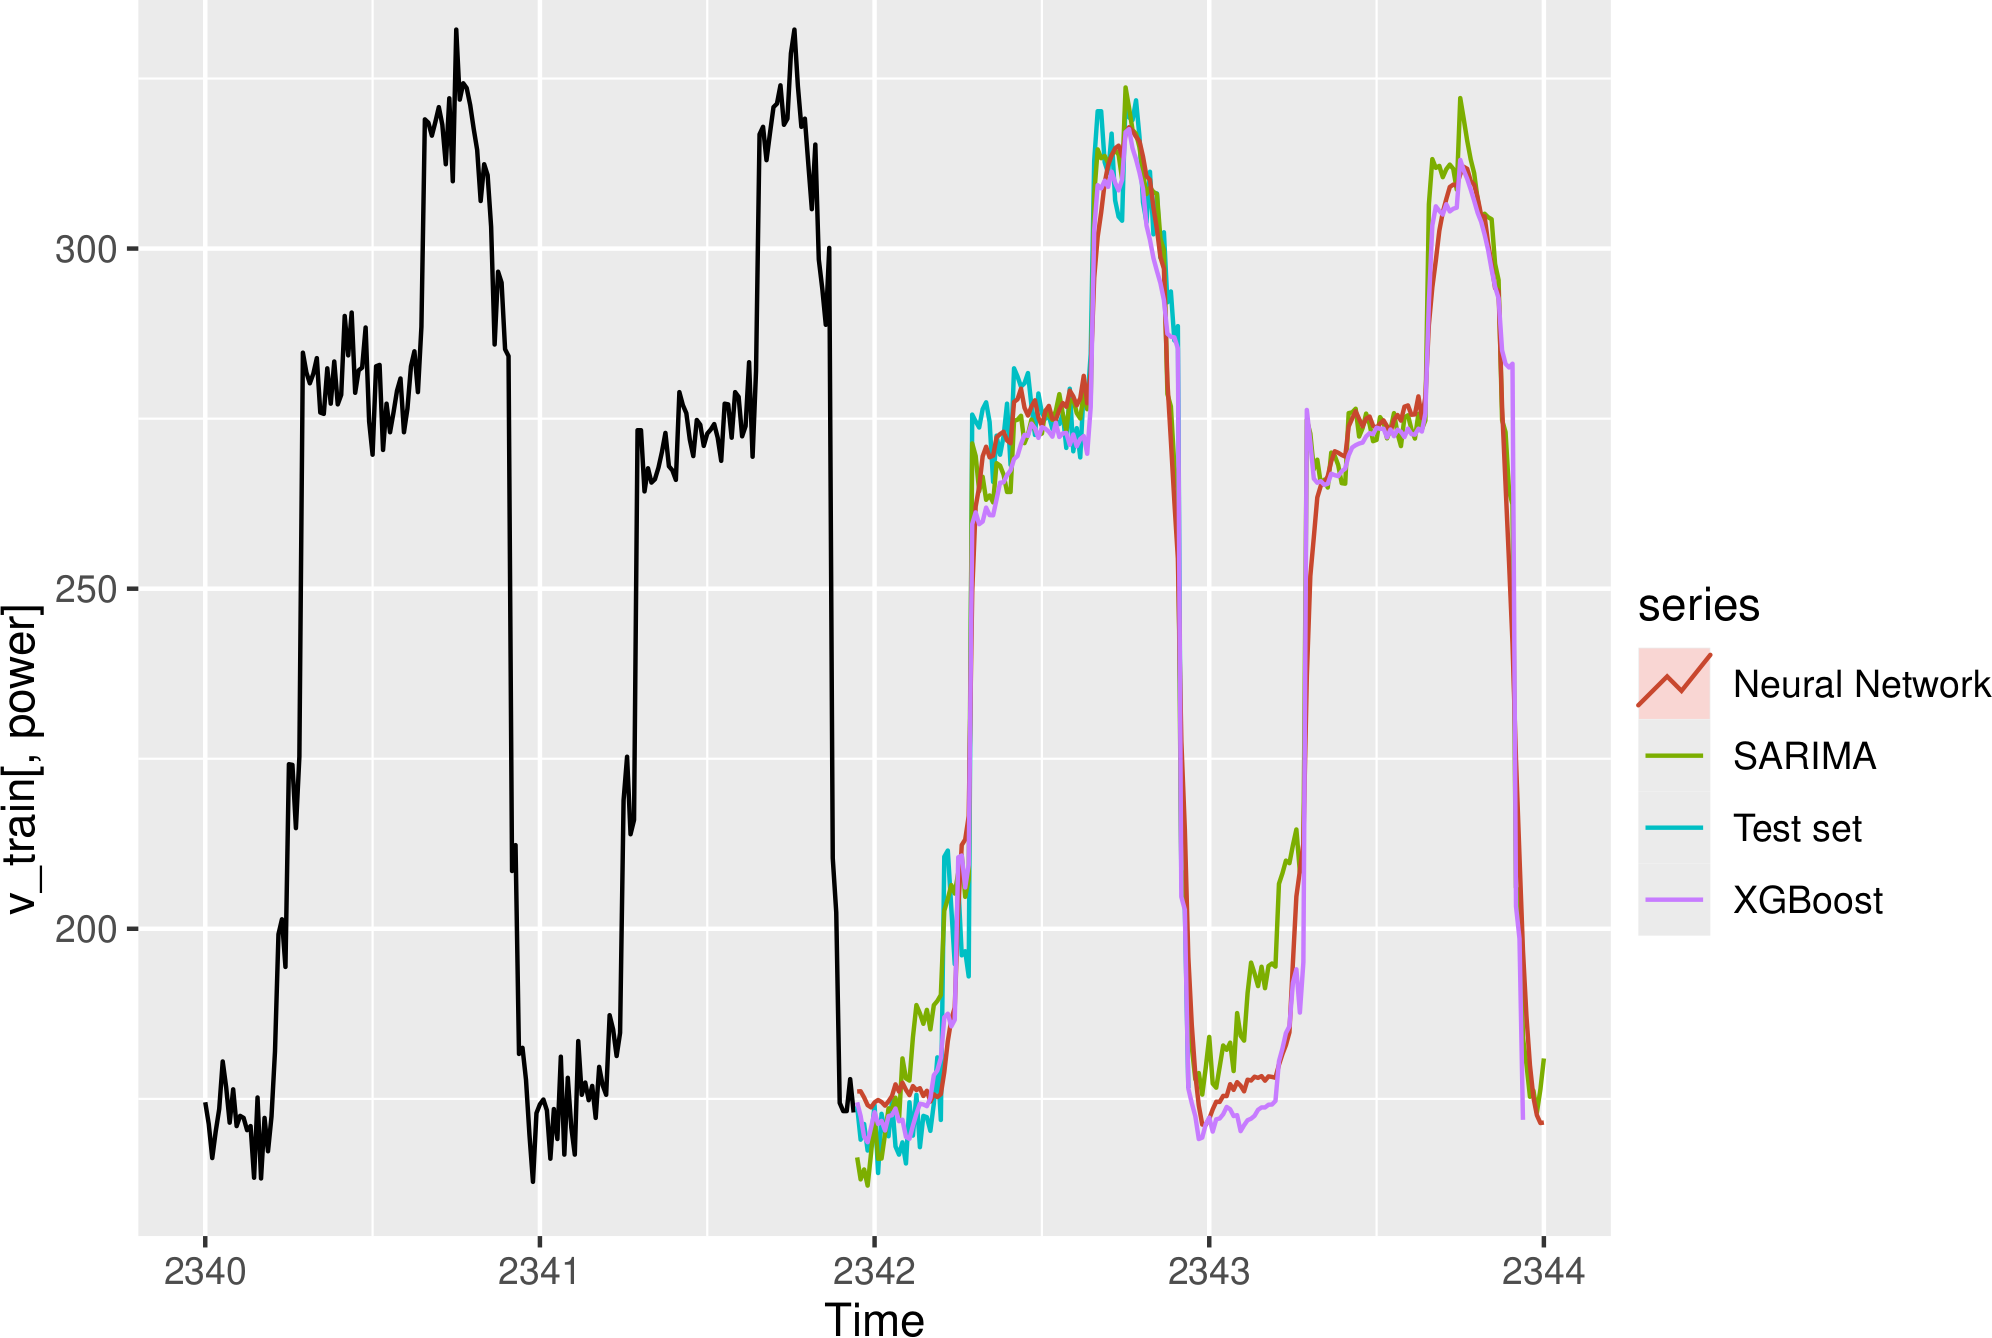
\includegraphics[scale=0.6]{figures/figure_discussion.png}
\caption{Modelling and forecast of electricity consumption.}
\label{figure_discussion}
\end{figure}

\red{\begin{itemize}
 \item with/with covariate : not much improvement
 \item XBGoost show best results in RMSE and computation time.
 \item all R code available in this file + github
\end{itemize}}
